\documentclass[letterpaper]{article} % DO NOT CHANGE THIS
\usepackage{aaai2027}  % DO NOT CHANGE THIS
% The serif, sans-serif, and monospaced fonts are loaded automatically by
% aaai2027.sty (newtxtext, helvet, courier). DO NOT add \usepackage{times},
% \usepackage{helvet}, \usepackage{courier}, or any other font package.
\usepackage[hyphens]{url}  % DO NOT CHANGE THIS
\usepackage{graphicx} % DO NOT CHANGE THIS
\urlstyle{rm} % DO NOT CHANGE THIS
\def\UrlFont{\rm}  % DO NOT CHANGE THIS
\usepackage{natbib}  % DO NOT CHANGE THIS AND DO NOT ADD ANY OPTIONS TO IT
\usepackage{caption} % DO NOT CHANGE THIS AND DO NOT ADD ANY OPTIONS TO IT
\frenchspacing  % DO NOT CHANGE THIS
%
% These are recommended to typeset algorithms but not required. See the subsubsection on algorithms. Remove them if you don't have algorithms in your paper.
\usepackage{algorithm}
\usepackage{algorithmic}

%
% Recommended for better-looking tables
\usepackage{booktabs}
\usepackage{multirow}
\PassOptionsToPackage{table}{xcolor}
\usepackage{amsfonts}
\usepackage{amsmath}

\usepackage[table,svgnames]{xcolor} % Added svgnames

%
% Keep the \pdfinfo as shown here. There's no need
% for you to add the /Title and /Author tags.
\pdfinfo{
/TemplateVersion (2027.1)
}

\setcounter{secnumdepth}{0} %May be changed to 1 or 2 if section numbers are desired.

% Convenience macros. The ladder is cumulative: each system is the previous
% one plus exactly one component, and its suffix names the LAST component it
% contains. Full GADAR is the top rung and carries no suffix.
\newcommand{\gadar}{GADAR}                 % + chain layer (top rung; the method)
\newcommand{\gadarstruct}{\gadar{}-STRUCT} % symbol-free structural features
\newcommand{\gadarbind}{\gadar{}-BIND}     % + lifted domain layer + binding layer
\newcommand{\union}{UNION}                 % control: symbol identity, D in weights
% Placeholder for results that do not exist yet - renders RED so no
% placeholder survives to submission unnoticed. Before submitting:
%   grep -c todonum gadar.tex   must print 0.
\newcommand{\todonum}[1]{\textcolor{red}{\textbf{[#1]}}}

\title{GADAR: Generalizing Across Domains via Action Ranking for Classical Planning}

% Anonymized for AAAI-27 review. Camera-ready author block below (commented).
\author{
    Anonymous Submission
}
\affiliations{
    Anonymized for review
}

\iffalse
% Camera-ready author block
\title{GADAR: Generalizing Across Domains via Action Ranking for Classical Planning}
\author {
    Rajesh Mangannavar
    % TODO: co-authors
}
\affiliations {
    Oregon State University\\
    Corvallis, OR 97330, USA\\
    mangannr@oregonstate.edu
}
\fi

\begin{document}

\maketitle

\begin{abstract}

Learned policies for classical planning act without search, but each is tied to the domain it was trained on: network modules per action schema, parameters per predicate, or vocabulary-sized encodings mean a trained policy cannot even be executed on a new domain's predicates and action schemas. We present \gadar{} (Generalizing Across Domains via Action Ranking), a policy that takes the domain description as input, $\pi(s, G, D)$, and constructs grounded actions in domains never seen in training, without search. Symbols are described by the roles they play in the domain rather than by their names, in three layers that each extend the previous one: (i) a \emph{lifted domain layer} embeds $D$ in every state graph through structural signatures; (ii) a \emph{binding layer} ties each ground action's applicability to the lifted preconditions it instantiates; and (iii) a \emph{chain layer} states which schema produces what another needs and how far each schema stands from the goal. We evaluate leave-one-domain-out over eight benchmark domains, selecting every checkpoint without access to the held-out domain. A single \gadar{} policy trained on seven domains solves 58.3\% of their test instances, trained on one domain it solves \todonum{--}\% against \todonum{--}\% for per-domain GABAR on the same instances, and a multi-task control that keeps symbol identity in its weights, while strong on some of the domains it trains on, transfers to none of the held-out ones. Zero-shot, \gadar{} executes on every held-out domain and solves \todonum{68}\% of the large test instances of held-out Visitall, where an identically-executed untrained network solves \todonum{0}\%. Transfer to the other seven held-out domains is limited (\todonum{0--5}\% on their test instances), and we identify where it fails: domains whose action schemas are structurally alike but play different roles, which renaming-invariant features cannot distinguish without data from the new domain.

\end{abstract}

% Uncomment the following to link to your code, datasets, an extended version or similar.
% You must keep this block between (not within) the abstract and the main body of the paper.
%\begin{links}
%    \link{Code}{https://aaai.org/example/code}
%    \link{Extended version}{https://aaai.org/example/extended-version}
%\end{links}

\section{Introduction}

Classical planning finds action sequences achieving goals in deterministic
environments. Traditional planners solve small problems optimally by search
and heuristics but scale poorly \citep{complexity-planning, fast_downward},
which motivates learning-based planning: a model trained on solved problems
captures regularities that carry over to new ones. Two families of learned
guidance have developed largely in parallel.
Learned \emph{heuristics} estimate cost-to-go and guide a search algorithm
\citep{strips_hgn, karia2021learning, goose_v2}; learned \emph{policies}
select actions directly, executing plans greedily without search
\citep{toyer2020asnets, expressive_v1, gabar}.

Learned policies generalize well \emph{within} a domain. ASNets learn
per-schema network modules that transfer across problem sizes
\citep{toyer2020asnets}; relational GNN policies learn value functions whose
greedy execution solves instances far larger than those seen in training
\citep{expressive_v1, policy_beyond_c2}; GABAR encodes states as
action-centric graphs and constructs grounded actions by ranking them
\citep{gabar}. All share a design choice: the domain's schemas and
predicates are reflected in the network itself, as modules, parameters, or
feature dimensions. Shaping the network to its domain aids within-domain
generalization, but it is also what binds each policy to that domain, which
cannot even be executed where its schemas and predicates have no slots.

For learned heuristics, a different treatment of the domain has emerged.
STRIPS-HGN computes structural features that make no reference to symbol
identity \citep{strips_hgn}, and GOOSE's lifted learning graph encodes the
full domain description as part of the heuristic's input, training one
heuristic across many domains and evaluating on held-out ones
\citep{goose_v2}. The input side of learning for planning can therefore be
made domain-agnostic. Heuristics, however, delegate action construction to
search; the corresponding step for policies, which must construct grounded
actions themselves, remains open, and \citet{goose_v2} name it as future
work. It is not a trivial step: the same authors prove that message passing
over the lifted graph cannot compute even $h^{\mathrm{add}}$, and their
domain-independent setting is empirically their hardest.

In this work we take that step, and our key idea is to change what the
network is told about symbols: not which symbol something is, but what role
the symbol plays in the domain. A predicate is described by where it
appears (which schemas require it, which produce or destroy it, at which
argument positions), and under that description gripper's
$\textsf{pick}$-then-$\textsf{drop}$ and miconic's
$\textsf{board}$-then-$\textsf{depart}$ are one structure, which a policy
can learn in one domain and reuse in another. Two things are then needed to
make the description usable: every ground action's applicability must be
tied to that structure, so that ``why is this action available'' is said in
the domain's own vocabulary; and the relation planning turns on, that one
schema produces what another needs, must be stated explicitly rather than
left for message passing to recover. The result is a policy
$\pi(s, G, D)$ that is at once domain-general and search-free, where
classical planners buy generality with search and learned policies buy
reactivity with specialization. The question we study is what such a policy
can transfer, not whether it outraces search.

We build this capability as a ladder of three systems, each adding one
group of representational commitments to the previous one, so that every
adjacent comparison isolates that group. \union{} is the control: symbol-identity
features widened to the union of the training vocabularies,
which is multi-task learning with the domain in the weights. \gadarbind{}
replaces symbol identity with structural features and puts $D$ into every
state graph, as a lifted domain layer plus the \emph{binding layer}.
Structure alone is not yet transfer: ``schema $A$ produces what schema $B$
consumes'' is only a two-hop path through a shared predicate hub, and the
hub loses the pairing. Full \gadar{} therefore adds the \emph{chain
layer}, stating that relation directly and marking how far each schema
stands from the goal. All three share one encoder, one ranking decoder, and the
same search-free execution, so every comparison varies the representation
and not the architecture.

Our experiments follow a leave-one-domain-out protocol over all eight
benchmark domains, with every checkpoint selected without access to the
held-out domain. \gadar{} executes on every held-out domain. On held-out
Visitall it solves \todonum{68}\% of the large test instances zero-shot at
plan quality \todonum{0.97}, against \todonum{0}\% for an
identically-executed untrained network, \todonum{0}\% for the
union-vocabulary control, and \todonum{4}\% without the chain layer. On the
other seven held-out domains transfer is limited, and the per-domain
results show where it breaks: when a held-out domain's schemas are
structurally alike but play different roles, as Logistics' truck and
airplane actions do, features that ignore symbol names cannot tell them
apart. \gadar{} is invariant by construction to renaming of predicates,
schemas, and objects, a robustness current large reasoning models lack
\citep{llm_baseline}; the same invariance means that what distinguishes
such schemas has to come from data in the new domain.

\textbf{Contributions.}
\begin{itemize}
\item To our knowledge, the first domain-agnostic \emph{policy} for
  classical planning: $\pi(s, G, D)$ constructs grounded actions zero-shot
  in unseen domains, without search.
\item A graph representation with two novel relations, both computable in
  any domain: \emph{binding} edges, which link each applicable ground
  action's objects to the lifted precondition occurrences they satisfy and
  so express why the action is applicable in the vocabulary of $D$, and \emph{chain} edges,
  which express which schema produces or destroys what another needs and
  how far each schema is from the goal.
%\item An evaluation designed as a ladder: each system is the previous plus   one component, so each component's contribution is measured directly, with matched untrained and multi-task controls under an identical execution harness.
\end{itemize}

\section{Related Work}


\textbf{Learning heuristics across domains.} Domain-independent heuristics
have a long history; we focus on the neural line. STRIPS-HGN trains
hypergraph networks on structural features of the delete relaxation and
evaluates on unseen domains \citep{strips_hgn}. GOOSE introduces graph
representations of planning tasks for grounded and lifted inputs; its
lifted learning graph encodes the domain description itself (schemas,
preconditions, effects, argument bindings via index features), and its
domain-independent setting trains one heuristic across many domains and
evaluates on held-out ones \citep{goose_v1, goose_v2}. WL-GOOSE obtains
stronger per-domain heuristics from Weisfeiler--Lehman features, at the
cost of per-domain feature dictionaries \citep{wl_goose}.
\citet{karia2021learning} learn generalized heuristics over canonical
abstractions; LLM-evolved heuristic ensembles transfer to a held-out IPC
learning track \citep{llm_evolved_heuristics_2026}. These works establish
domain-agnostic inputs, and we adopt their lesson of structural features
and lifted domain graphs. They differ in output: a heuristic delegates
action construction to search, which stays in the execution loop.
\citet{goose_v2} further prove an expressiveness limitation of message
passing on their lifted graph and name lifted policy learning as open; our
binding layer adds exactly the information a policy needs and their graph
provably lacks (their Theorem 4.3).

\textbf{Learned policies for planning.} Generalized policy learning aims at
policies that transfer across instances of a domain
\citep{approx_Policy_iter, relational_rl}. ASNets construct a network from
the domain's action schemas and ground atoms, with weight sharing across
instantiations of the same schema \citep{toyer2020asnets}. St{\aa}hlberg,
Bonet, and Geffner learn value functions with GNNs whose greedy policies
generalize across instance sizes, characterize their expressive power in
terms of two-variable logics, and extend the approach with policy gradients
and unsupervised objectives \citep{expressive_v1, unsupervised_gnn,
policy_gradients, policy_beyond_c2}. Relational deep RL approaches
similarly learn policies over relational state representations
\citep{relational_drl, sr_drl, relational_mdp_learning, rddl_gnn,
generalized_planning_deep_rl}. GABAR represents ground actions explicitly in the
state graph and constructs actions autoregressively by ranking
\citep{gabar}. The same action-centric idea extends beyond full
observability: GammaZero converts particle beliefs into uncertainty-aware
graphs to guide belief-space search \citep{gammazero}, which opens the
approach to tasks such as object rearrangement under partial observation
\citep{hoo_pomdp}. That line relaxes what the policy can observe while
holding the domain fixed; we do the opposite, keeping the classical
fully observable setting and varying the domain. The most recent work remains per-domain: self-improving
search-and-learn loops train a relational value heuristic per domain
\citep{learning_to_search_2026}, lookahead-based general policies are
learned over instances of a single domain
\citep{lookahead_policies_2026}, and Q-value policy learning is framed
per-domain explicitly \citep{mueller_qvalues}. In all of these the
vocabulary lives in the network as per-schema modules, per-predicate
parameters, or vocabulary-sized encodings, binding the policy to its
training domain. \gadar{} removes that binding by moving the domain
description from the network's parameters into its input.

\textbf{Ranking in planning.} Learning to rank has ordered states and
heuristic values for search \citep{ranking_old_2009, ranking_og,
chrestien_optimize, gbfs_v2}; GABAR instead ranks \emph{actions} locally
within a state \citep{gabar}. Cross-domain, this choice becomes
load-bearing: a shared value function presupposes a common scale of goal
distances that does not exist across domains, whereas local rankings are
scale-free. \citet{mueller_qvalues} report convergent evidence: Q-value
regression fails for lack of action discrimination and a ranking-style
margin repairs it.

\textbf{Large language models and planning.} Large reasoning models degrade
sharply under symbol renaming \citep{llm_baseline}, an invariance \gadar{}
has by construction. LLM pipelines that synthesize per-domain programs or
generate and repair PDDL across domains \citep{halo_orchestrator} operate
at the specification level and leave planning to search, which is a
different question from zero-shot policy execution.

\section{Background and Problem Setup}

A classical planning problem $P = \langle D, I \rangle$ pairs a first-order
domain $D$ (predicate symbols $\mathcal{P}$ with arities, and action
schemas $\mathcal{A}$, each with parameters, preconditions $pre(a)$, and
add/delete effects $add(a)$, $del(a)$) with instance information
$I = \langle O, s_0, G \rangle$: objects, an initial state, and a goal
condition, the last two as sets of ground atoms. A ground action
substitutes objects for a schema's parameters, is applicable in $s$ if
$pre(a) \subseteq s$ under the substitution, and yields
$s' = (s \setminus del(a)) \cup add(a)$; a plan is an applicable sequence
from $s_0$ to a state satisfying $G$.

GABAR learns, per domain, a policy $\pi_D(s, G)$ that generalizes to larger
instances of the \emph{same} domain \citep{gabar}. We address the
cross-domain version: from solved small instances of training domains
$D_1, \dots, D_n$, learn a \emph{single} policy $\pi(s, G, D)$, with the
domain description itself an input, that solves instances of a test
domain $D_{\mathit{test}} \notin \{D_1, \dots, D_n\}$, zero-shot. Execution
is search-free: the highest-ranked applicable action is executed, a monitor optionally avoids revisiting states, and execution ends
at the goal, a dead end, or a length bound.

\begin{figure*}[t]
\centering
% Source: figures/fig1_representation.html, updated 2026-07-28 with the
% chain layer (enables edge, grounded deletes-true edge, goal-relevant object
% rings, chain legend block). PNG rendered headlessly 2026-07-28 and committed
% (no manual screenshot needed; re-render: tools note in figures/).
% the SVG area only, save on Overleaf as Figures/gadar_graph_v1.png).
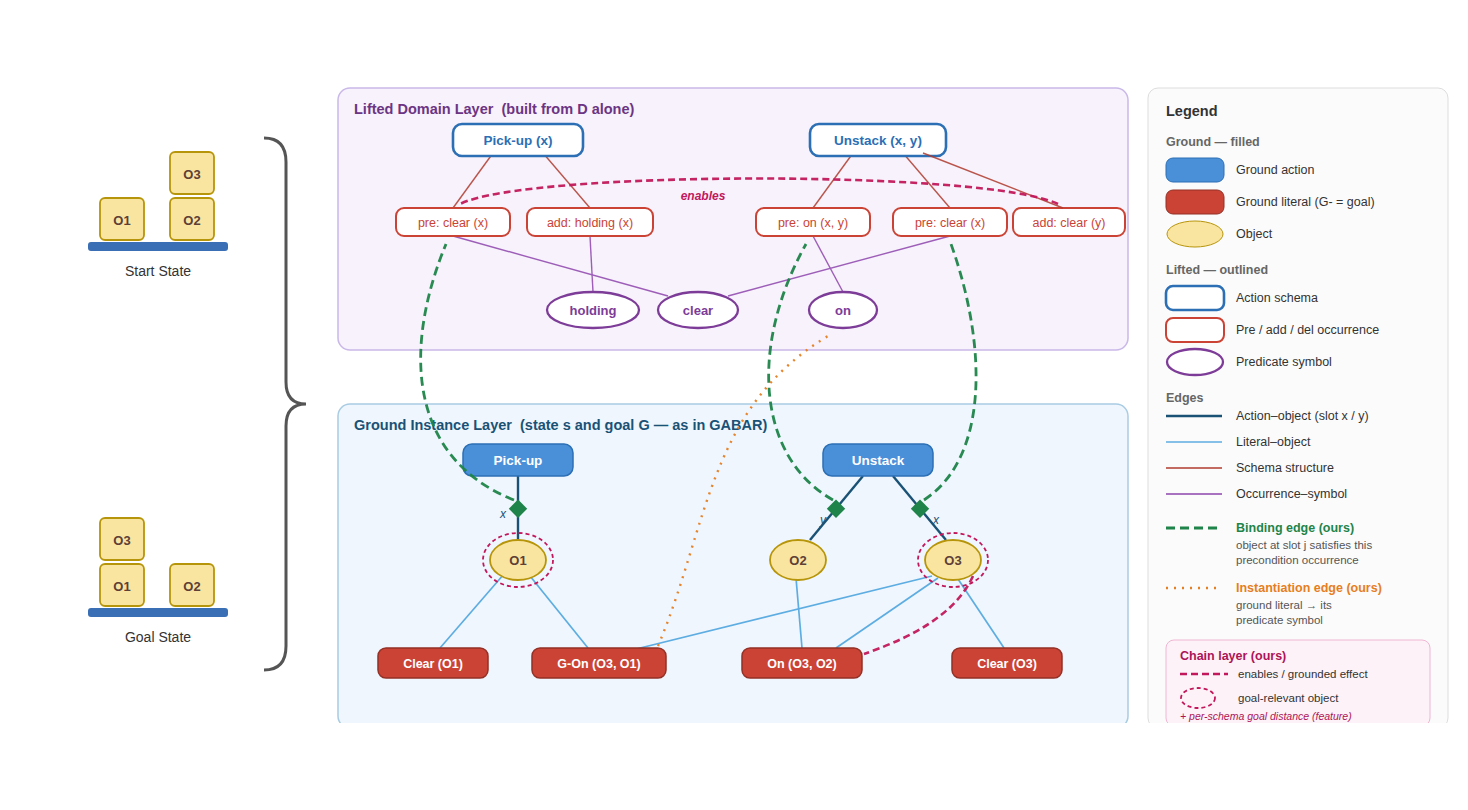
\includegraphics[width=0.98\textwidth]{Figures/gadar_graph_v1.png}
\caption{The \gadar{} representation for a Blocksworld task. The
\emph{ground instance layer} (bottom) is the action-centric graph of the
grounded policy we build on \citep{gabar}: objects, ground literals of the state and goal (G- prefix), and ground
action nodes with action--object edges carrying parameter slots. The
\emph{lifted domain layer} (top) is built from $D$ alone: schemas, their
precondition and effect occurrences, and predicate symbols. \emph{Binding
edges} (green, dashed) link an object's slot on an applicable ground action
to the precondition occurrences it satisfies; \emph{instantiation edges}
(orange, dotted) link each ground literal to its predicate symbol. Filled
nodes are ground, outlined nodes lifted. \union{} uses the ground layer
with symbol-identity features; \gadarbind{} makes them structural and adds
the lifted layer and binding edges; \gadar{} adds the chain layer
(magenta), shown as one exemplar each of an \emph{enables} edge, a grounded
deletes-true edge, and goal-relevance rings. No feature encodes symbol
identity, so the representation is renaming-invariant by construction.}
\label{fig:representation}
\end{figure*}

\begin{figure*}[t]
\centering
% Source: figures/fig2_system.html. Redrawn 2026-07-29: text in the ladder
% cut to one line per rung and fonts enlarged for column-width legibility;
% canvas 1420x540, fonts scaled up again 2026-07-29 now that the page has
% vertical room. PNG rendered headlessly (chromium via playwright,
% device_scale_factor=3) and committed.
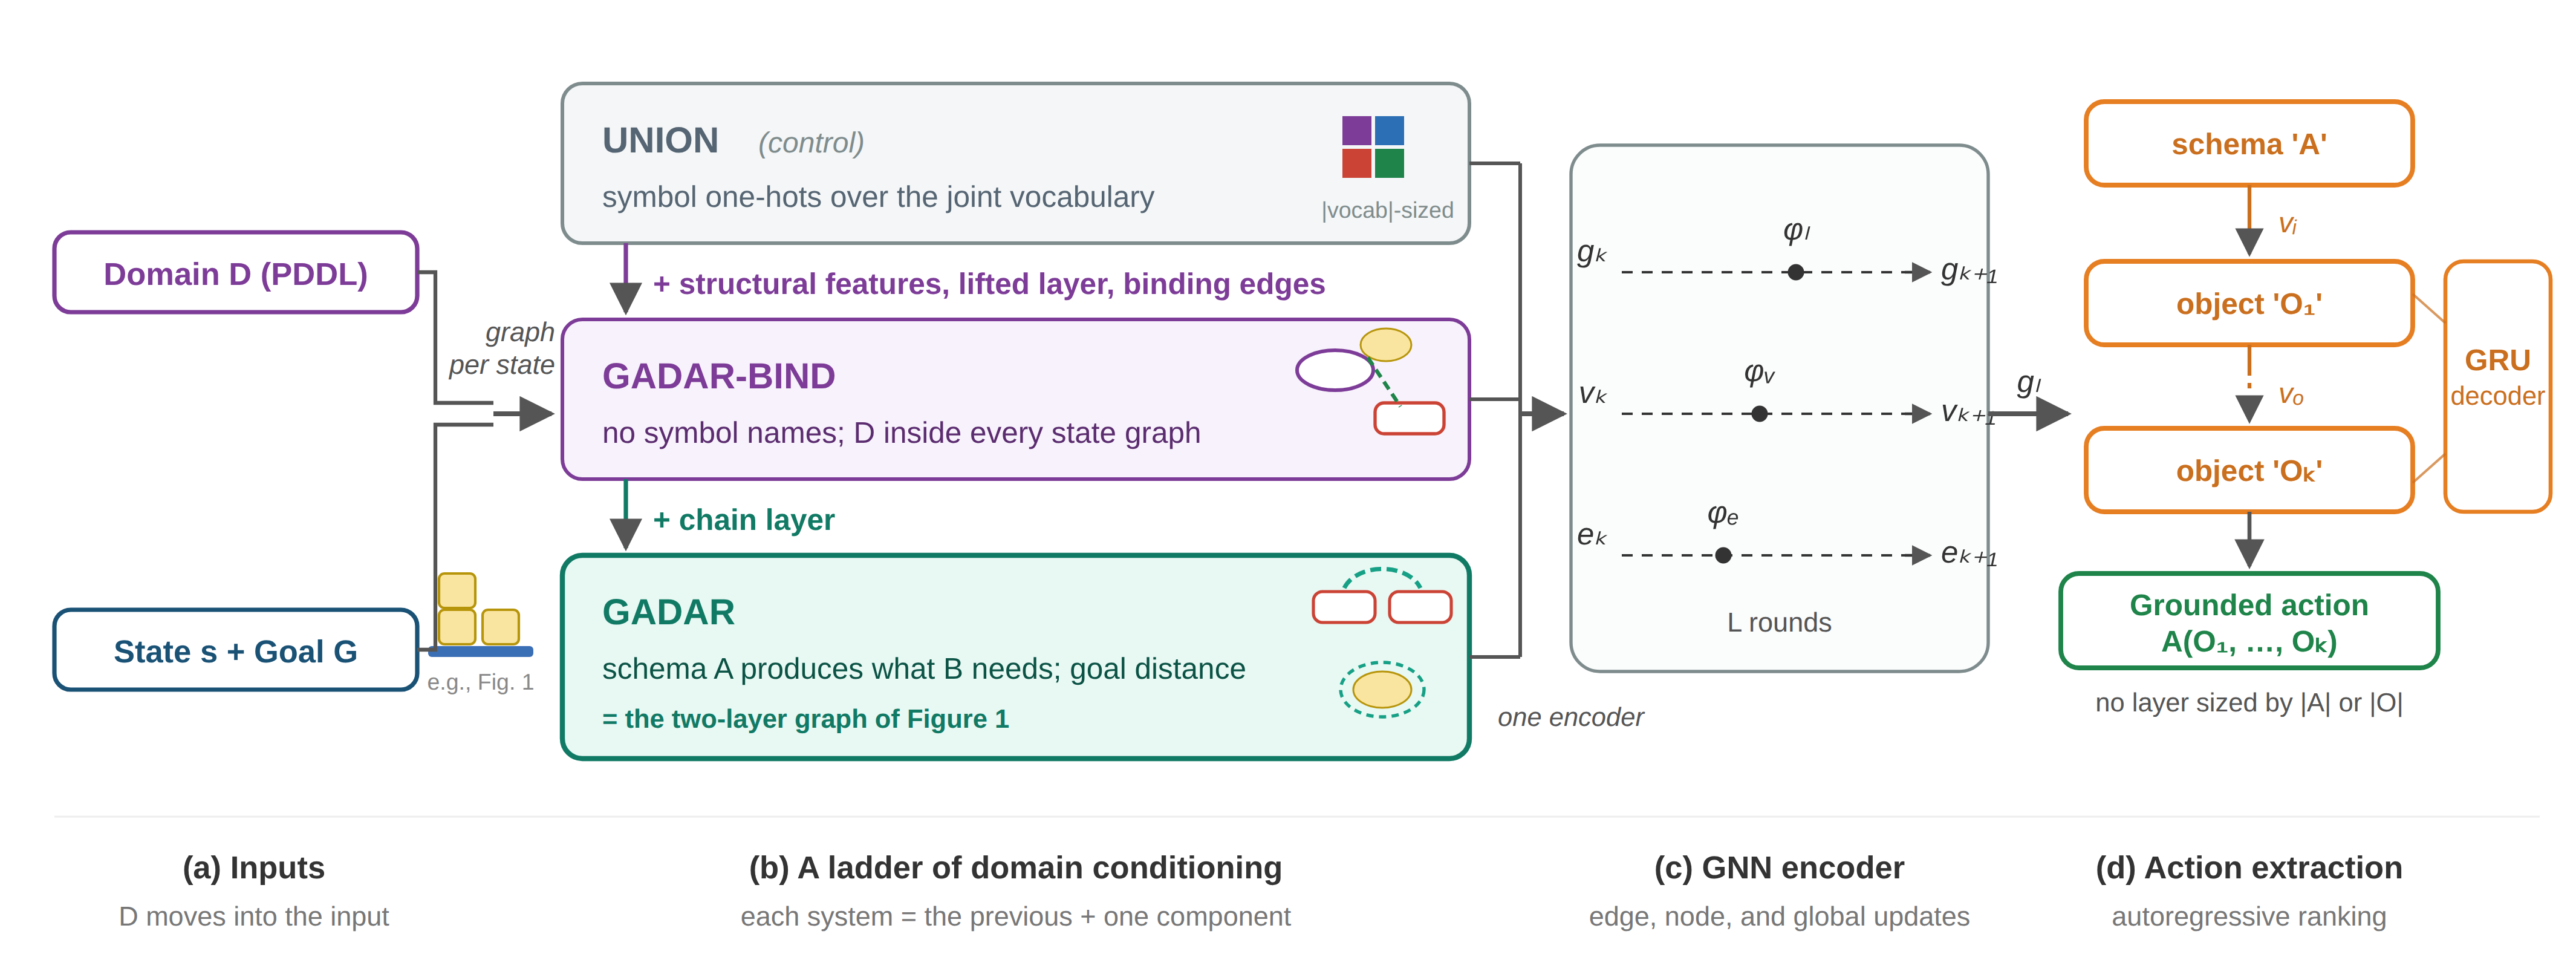
\includegraphics[width=1.0\textwidth]{Figures/gadar_system_v1.png}
\caption{\gadar{} system overview. (a) $D$, the state, and the goal are
converted into a graph. (b) The ladder of domain conditioning, three
systems each the previous plus one commitment: \union{} (symbol one-hots
over the joint vocabulary), \gadarbind{} (structural features, lifted
domain layer, binding layer of Figure~\ref{fig:representation}), \gadar{}
(chain layer). Every adjacent comparison isolates one component. (c) The
GNN encoder, $L$ rounds of edge, node, and global updates. (d) The GRU
decoder constructs a grounded action autoregressively,
schema then arguments, by scoring schema- and object-node embeddings; no
component is sized by the number of schemas or objects.}
\label{fig:system}
\end{figure*}

\section{GADAR}

Given a planning instance in PDDL format together with its domain
description $D$, \gadar{} converts the pair into a graph, processes the
graph with a GNN encoder, and constructs a grounded action with a GRU-based
decoder that first selects an action schema and then each of its arguments
(Figure~\ref{fig:system}). Encoder and decoder are those of the per-domain
policy of \citet{gabar}, summarized here for completeness; what changes is
the graph they operate on. We present the representation as it is
evaluated: a ladder of systems in which each addition is measured against
its predecessor.

\textbf{Encoder.} Node, edge, and global features are first embedded by
separate MLPs into $d{=}64$ dimensions. Each of $L{=}9$ rounds then (1)
updates every edge from its two endpoints, its own embedding, and the global
node, (2) updates every node from its incoming edges, aggregated by
attention (a softmax over the node's incoming edges), and (3) updates the
global node from all nodes and edges. At every round the current embeddings
are concatenated with their round-0 encodings before the update, a skip
connection that keeps the input features visible at depth. The output is
one embedding per node, which the decoder ranks.

\subsection{A Domain-Agnostic Graph Representation}

\textbf{Ground instance layer.} The base of the representation is that
action-centric graph: nodes for objects, for ground literals
of the current state and the goal (goal literals marked by a flag), and for
action schemas, together with a global node; edges connect literals to their
argument objects and schemas to the objects of their applicable groundings,
with parameter positions on the edges (Figure~\ref{fig:representation},
bottom). This graph is what makes search-free action construction possible:
the decoder selects among schema nodes and object nodes that are present in
the input.

\textbf{The graph.} A task $(s, G, D)$ is encoded as
$\mathcal{G} = (V, E, X, R)$. The node set is
\begin{equation*}
V \;=\; O \,\cup\, L \,\cup\, A \,\cup\, \Sigma \,\cup\, Q \,\cup\, \{g\},
\end{equation*}
where $O$ are the objects, $L$ the ground literals of the state and goal,
$A$ the action schemas (one node per schema), $\Sigma$ the
predicate symbols of $D$, including one synthetic unary static predicate
per declared type so that typed and predicate-typed domains present the
same structure, $Q$ the \emph{occurrence nodes} $q_{a,k}$, one per
literal occurrence $k$ in the preconditions and effects of schema $a$, and
$g$ a global node. The edge set is a union of typed relations,
\begin{equation*}
E \;=\; E_{\mathrm{lit}} \cup E_{\mathrm{act}} \cup E_{\mathrm{inst}} \cup
E_{\mathrm{occ}} \cup E_{\mathrm{bind}} \cup E_{\mathrm{chain}} \cup
E_{\mathrm{eff}},
\end{equation*}
\begin{itemize}
\item $E_{\mathrm{lit}} \subseteq L \times O$, $E_{\mathrm{act}} \subseteq
  A \times O$: literals to their arguments and schemas to the objects of
  their \emph{applicable} groundings (the ground layer), with argument
  and slot positions as edge features;
\item $E_{\mathrm{inst}} \subseteq (L \cup O) \times \Sigma$:
  \emph{instantiation}, each literal to its predicate's symbol and each
  object to its declared type's symbol;
\item $E_{\mathrm{occ}} \subseteq Q \times (\Sigma \cup A)$: each occurrence
  to its predicate symbol and to its schema, carrying the role
  $r(q) \in \{\mathrm{pre}, \mathrm{add}, \mathrm{del}\}$ and the
  argument-to-slot pairs $(i, j)$ of that occurrence;
\item $E_{\mathrm{bind}} \subseteq O \times Q$, the \emph{binding layer}:
  $(o, q_{a,k})$ whenever some applicable grounding of $a$ places $o$ at a
  slot that occurrence $k$ constrains;
\item $E_{\mathrm{chain}} \subseteq Q \times Q$, the \emph{chain layer}:
  $\textit{enables} = \{(q, q') : r(q) = \mathrm{add},\, r(q') =
  \mathrm{pre},\, \mathrm{pred}(q) = \mathrm{pred}(q')\}$ and
  \textit{threatens} likewise with $r(q) = \mathrm{del}$;
\item $E_{\mathrm{eff}} \subseteq O \times L$, the grounded effect edges: for
  each applicable grounding, an instantiated add effect equal to an
  \emph{unsatisfied} goal atom $\ell$ (\textit{achieves-goal}), or a delete
  effect equal to a \emph{true} atom $\ell$ (\textit{deletes-true}), links
  the grounding's objects to $\ell$.
\end{itemize}
Node features $X : V \to \{0,1\}^{d}$ concatenate indicator segments: the
node's kind; the arity (clamped at global caps $k_p$, $k_a$) and a
static-predicate flag; a goal flag on literals; on schema nodes the
goal-distance one-hot $\mathrm{gdist}(a) \in \{0, 1, 2, 3{+}\}$, the BFS
depth over \textit{enables} from the schemas that add a goal predicate; and
on objects a goal-relevance bit (the object occurs in an open goal atom).
Edge features $R : E \to \{0,1\}^{k}$ concatenate the relation type with
position, slot, and role indicators up to the caps. The widths $d$ and $k$
are functions of $(k_p, k_a)$ alone; no dimension is $|A|$, $|P|$,
$|T|$, or $|O|$. A single network therefore serves every domain, instances from
different domains batch together, and permuting symbol names leaves
$(X, R)$ unchanged: renaming invariance holds by construction. Every
feature is a flag or a one-hot; nothing is a magnitude. The goal distance
in particular is bucketed rather than numeric, deliberately: a number must
be read on a scale, and no scale is shared across domains. The same
argument makes local action ranking, rather than value regression, the
right objective in this setting.

\textbf{Cost.} $\Sigma$, $Q$, $E_{\mathrm{occ}}$, and $E_{\mathrm{chain}}$
are domain-sized constants computed once per domain; $\mathrm{gdist}$
depends only on which predicates occur in the goal and is computed once per
(domain, goal signature). Only $E_{\mathrm{bind}}$, $E_{\mathrm{eff}}$, and
the goal marks are per-state, each linear in the applicable groundings and
open goal atoms.

\textbf{Why these relations.} $E_{\mathrm{bind}}$ connects what the two
prior lines capture only separately: LLG has lifted preconditions but no
ground actions, and GABAR has ground applicability but indexed by
per-domain strings that do not transfer. Binding expresses why each action is applicable in $D$'s own
vocabulary.\footnote{Binding edges are \emph{cross-layer}: each joins a
node of the ground instance layer (an object of the current problem) to one
of the lifted domain layer (a precondition occurrence of a schema in $D$).
The graph contains both layers; the binding edges connect them.} In
Figure~\ref{fig:representation}, the edge placing O3 in Unstack's first
slot binds to the occurrences \emph{on(x,y)} and \emph{clear(x)}, and this
information survives unchanged if every symbol is renamed.
$E_{\mathrm{chain}}$ states directly that schema $A$ produces what schema
$B$ needs. Without it, this relation exists only as a two-hop path through
a shared predicate hub, and the hub's aggregation destroys the
producer--consumer pairing. Because the chain edges connect occurrences,
the pairing survives message passing, delete effects acquire a consequence,
and the relation transfers across domains: gripper's
$\textsf{pick} \rightarrow \textsf{drop}$ and miconic's
$\textsf{board} \rightarrow \textsf{depart}$ are the same structure, an
\textit{enables} edge between an add- and a pre-occurrence of a shared
predicate. $E_{\mathrm{eff}}$ grounds the layer: the decoder scores object
nodes, and these edges place ``this object closes an open goal'' and ``this
object undoes something true'' one hop from the quantity being ranked.


\textbf{Relation to GOOSE's LLG.} LLG and our lifted layer share the essential idea of the domain
description as input, and differ in encoding: argument positions as edge
features rather than chains of index nodes, and occurrence nodes carrying
exact argument-to-slot pairs. The fundamental difference is purpose. A
heuristic graph must support one number read from a global embedding, so
LLG contains no ground actions and no applicability information, and
\citet{goose_v2} prove message passing on it cannot compute
$h^{\mathrm{add}}$. A policy graph must contain the decoder's targets, the
schema and object nodes to score, and the evidence for scoring them: which
groundings are applicable and why. The binding layer supplies that evidence
in $D$'s own vocabulary.

\subsection{A Ladder of Domain Conditioning}

The three systems stand in a strict subset relation. \union{} (control)
keeps the symbol-identity one-hots, widened to the union of the training
vocabularies: the domain stays in the weights, which is multi-task
learning, not domain conditioning. \gadarbind{} replaces those one-hots
with the structural features $X$, making the policy executable in any
domain, and adds $\Sigma$, $Q$, $E_{\mathrm{inst}}$, $E_{\mathrm{occ}}$,
and $E_{\mathrm{bind}}$. \gadar{} adds $E_{\mathrm{chain}}$,
$E_{\mathrm{eff}}$, and the goal-distance and goal-relevance features.
Because adjacent systems differ in one group of components, the experimental
comparison and the ablation study are the same object: the
\union{}-to-\gadarbind{} step measures what removing symbol identity costs
and what the domain description buys, and the \gadarbind{}-to-\gadar{}
step measures the chain layer together with the grounded effect edges and
goal features it adds. We do not separate those three here, and attribute
the second step to them jointly.

\subsection{Action Construction and Training}

The decoder changes only where per-domain constants would otherwise appear
(Figure~\ref{fig:system}d). A GRU selects a schema by
scoring schema-node embeddings against its hidden state, then each argument
in turn by scoring object-node embeddings, feeding every selection back as
the next input. The argument loop runs to the selected schema's arity, read
from $D$ under a global arity cap rather than a per-domain constant. No
component is sized by the number of schemas, objects, or predicates;
selection is always a dot product between the decoder state and the
embedding of a node present in the graph, which is what lets one network
construct actions in a domain whose schemas it has never seen. Training is
supervised: cross-entropy against the expert's schema and argument
choices at every state along planner-generated plans. Because
feature widths are domain-independent, domains mix freely within a
batch.

\section{Experimental Setup}

\textbf{Domains.} We evaluate on the eight benchmark domains used by GABAR:
Blocks, Miconic, Spanner, Gripper, Visitall, Grid, Logistics, and
Rovers \citep{gabar, pddl-generators}. Training data consists of plans
computed by Fast Downward with the LAMA-first satisficing configuration
\citep{fast_downward} on the small instances of each training domain
(between 125 and 312 instances per domain); states along each plan are
converted to graphs and the policy is trained to reproduce the expert
action as described above. Every one of the eight domains serves as a
held-out target, each on two splits.

\textbf{Protocol.} Two experiment families, run for every rung of the
ladder. (i)~\emph{Leave-one-domain-out} (the main experiment): for each of
the eight domains, a policy is trained on the remaining seven and evaluated
on the held-out domain zero-shot, having never seen its predicates,
schemas, or objects. (ii)~\emph{In-domain}: the same seven-domain policies
are evaluated on the domains they trained on, and for each domain we report
the mean over the seven policies whose training set includes it; a
single-domain variant, \gadar{}$_1$, trains the same representation on that
domain alone. The \emph{hard} split is the domain's test
set, with instances up to an order of magnitude larger than training-scale
problems; the \emph{easy} split is the held-out domain's own
training-scale instances, unseen because the domain was held out, which
separates failing on the unseen domain from failing to scale within it.
Training domains are evaluated on the hard split only.

\textbf{Checkpoint selection.} No choice uses the held-out domain.
In-domain results use the checkpoint with the lowest combined training and
validation loss. For zero-shot results the training epoch is a
hyperparameter selected across folds: for held-out domain $d$, we use the
epoch $e^*(d)$ that maximizes mean zero-shot coverage on the hard splits of
the \emph{other} seven held-out domains, each measured with its own fold's
model; $d$'s own instances never enter the choice. The same rule is applied
to every rung. Each configuration is trained with a single seed, so we do
not report variance across seeds.

\textbf{Baselines and references.} Our primary comparison is the \union{}
control described above: identical data, architecture, and training
procedure, with only the representation different. Any zero-shot
capability \gadar{} has beyond this control comes from moving the domain
into the input. Two floors bound the zero-shot numbers from below. The
\emph{random floor} is the same executor and monitor choosing uniformly
among applicable ground actions, averaged over three rollouts per problem;
it measures how far legal moves alone get on each split. The
\emph{untrained control} is the identical system, with the same graph,
decoder, executor, and step bound, but a network that has seen a single
epoch of training. As a reference for dedicated training we report
published per-domain GABAR \citep{gabar}, trained directly on each
held-out domain and evaluated on its own test instances, averaged over its
three published size bands. Those instances are not identical to ours, so
GABAR$^\dagger$ indicates what per-domain training achieves at this scale
rather than serving as a matched comparison. For a matched comparison we
also retrain per-domain GABAR through our pipeline on Blocks, Gripper, and
Miconic, evaluated on exactly our test instances with the same checkpoint
rule (GABAR in Table~\ref{table:indomain}).

\textbf{Ablations and oracle.} The ladder is the ablation study
(Figure~\ref{fig:system}b), and each group of components is measured by
adjacent columns of Table~\ref{table:main_table}. We additionally report
one diagnostic that is not a rung of the ladder: an \emph{achievement
oracle} that, at every state, prefers any applicable ground action whose
add effects directly satisfy an unsatisfied goal atom, and otherwise defers
to the policy. It bounds what a hand-coded terminal trigger can achieve on
each domain.

\textbf{Metrics and implementation.} We report coverage (C), the
percentage of test problems solved within a 500-step bound, and
plan quality (P), the ratio of the reference planner's plan length to the
policy's on jointly solved problems, so values above 1 mean plans shorter
than the reference. Because P conditions on what a system solves, higher
coverage is scored on harder instances; coverage is the primary metric and
P is compared within, not across, columns. Encoder and decoder
hyperparameters are carried over unchanged ($L{=}9$
message-passing rounds, 64-dimensional representations, GRU decoder), with
batch size 64 and learning rate $5{\times}10^{-4}$, for 500 epochs; the
appendix lists every final setting. One seven-domain model takes
\todonum{about 14} hours to train on a single GPU, and one single-domain
model between half an hour and two hours. Renaming invariance is
verified as a unit test: permuting all symbol names in a domain yields
identical input tensors.

\section{Results and Discussion}

Table~\ref{table:main_table} presents the zero-shot results for all eight
held-out domains, and Table~\ref{table:indomain} the in-domain results. We
organize the discussion so that each question is answered by one
comparison: a rung of the ladder, a control, or a diagnostic.

\begin{table}[t]
\setlength{\tabcolsep}{2.2pt}
\renewcommand{\arraystretch}{1.05}
\footnotesize
\centering
\caption{Zero-shot coverage (C, \%) leave-one-domain-out: each row's domain
is held out of training. E = the held-out domain's own training-scale
instances (unseen); H = its test instances, up to an order of magnitude
larger. Rand: uniform choice among applicable actions under the same
executor and monitor (mean of three rollouts). Untr: the identical system
after one epoch of training. Ladder columns add one group of components
each: \union{} (symbol one-hots, domain in the weights), \gadarbind{}
(structural features, lifted domain layer, binding edges), \gadar{} (chain
layer, effect edges, goal features). P: \gadar{}'s plan quality.
GABAR$^\dagger$: published per-domain GABAR, trained \emph{on} the domain
and evaluated on its own test instances (not identical to ours).}
\label{table:main_table}
\begin{tabular}{@{}ll|cc|ccc|c|c@{}}
\toprule
Domain & & Rand & Untr & \union{} & \gadarbind{} & \textbf{\gadar{}} & P & GABAR$^\dagger$ \\
\midrule
\multirow{2}{*}{Blocks}    & E & 1.7  & \todonum{--} & \todonum{--} & \todonum{--} & \todonum{17.5} & \todonum{--} & -- \\
                           & H & 0.2  & \todonum{--} & \todonum{--} & \todonum{--} & \todonum{4.5}  & \todonum{--} & 100.0 \\
\midrule
\multirow{2}{*}{Gripper}   & E & 0.0  & \todonum{--} & \todonum{--} & \todonum{--} & \todonum{0.0}  & -- & -- \\
                           & H & 0.0  & \todonum{--} & \todonum{--} & \todonum{--} & \todonum{0.0}  & -- & 100.0 \\
\midrule
\multirow{2}{*}{Miconic}   & E & 88.3 & \todonum{2.6} & \todonum{--} & \todonum{--} & \todonum{2.6} & \todonum{--} & -- \\
                           & H & 1.1  & \todonum{--} & \todonum{--} & \todonum{--} & \todonum{0.0}  & -- & 100.0 \\
\midrule
\multirow{2}{*}{Visitall}  & E & 99.7 & \todonum{26.4} & \todonum{--} & \todonum{--} & \todonum{100.0} & \todonum{0.81} & -- \\
                           & H & 6.0  & \todonum{0.0} & \todonum{--} & \todonum{--} & \todonum{\textbf{68.0}} & \todonum{0.97} & 90.7 \\
\midrule
\multirow{2}{*}{Grid}      & E & 3.0  & \todonum{--} & \todonum{--} & \todonum{--} & \todonum{13.0} & \todonum{--} & -- \\
                           & H & 0.0  & \todonum{--} & \todonum{--} & \todonum{--} & \todonum{0.0}  & -- & 96.3 \\
\midrule
\multirow{2}{*}{Logistics} & E & 0.0  & \todonum{--} & \todonum{--} & \todonum{--} & \todonum{0.0}  & -- & -- \\
                           & H & 0.0  & \todonum{--} & \todonum{--} & \todonum{--} & \todonum{0.0}  & -- & 79.0 \\
\midrule
\multirow{2}{*}{Spanner}   & E & 63.4 & \todonum{--} & \todonum{--} & \todonum{--} & \todonum{0.0}  & -- & -- \\
                           & H & 43.8 & \todonum{--} & \todonum{--} & \todonum{--} & \todonum{0.0}  & -- & 92.0 \\
\midrule
\multirow{2}{*}{Rovers}    & E & 75.2 & \todonum{--} & \todonum{--} & \todonum{--} & \todonum{0.0}  & -- & -- \\
                           & H & 30.9 & \todonum{--} & \todonum{--} & \todonum{--} & \todonum{0.0}  & -- & 82.0 \\
\bottomrule
\end{tabular}
\end{table}

\begin{table}[t]
\setlength{\tabcolsep}{4pt}
\renewcommand{\arraystretch}{1.1}
\small
\centering
\caption{In-domain coverage (hard split). \union{}, \gadarbind{},
\gadar{}: mean over the seven leave-one-out policies whose training set
includes the domain; each policy serves seven domains. \gadar{}$_1$: the
same representation trained on that domain alone. GABAR: per-domain GABAR
retrained through our pipeline, on the same test instances.
GABAR$^\dagger$: published per-domain GABAR on its own test instances.}
\label{table:indomain}
\begin{tabular}{@{}l|cc|ccc|c@{}}
\toprule
Domain & GABAR$^\dagger$ & GABAR & \union{} & \gadarbind{} & \gadar{} & \gadar{}$_1$ \\
\midrule
Blocks    & 100.0 & \todonum{--} & \todonum{--} & \todonum{--} & 74.6 & \todonum{--} \\
Miconic   & 100.0 & \todonum{--} & \todonum{--} & \todonum{--} & 61.9 & \todonum{--} \\
Gripper   & 100.0 & \todonum{--} & \todonum{--} & \todonum{--} & 94.5 & \todonum{--} \\
Spanner   & 92.0  & --           & \todonum{--} & \todonum{--} & 47.9 & \todonum{--} \\
Visitall  & 90.7  & --           & \todonum{--} & \todonum{--} & 81.1 & \todonum{--} \\
Grid      & 96.3  & --           & \todonum{--} & \todonum{--} & 94.6 & \todonum{--} \\
Logistics & 79.0  & --           & \todonum{--} & \todonum{--} & 2.7  & \todonum{--} \\
Rovers    & 82.0  & --           & \todonum{--} & \todonum{--} & 9.0  & \todonum{--} \\
\midrule
Mean      & 92.5  & \todonum{--} & \todonum{--} & \todonum{--} & 58.3 & \todonum{--} \\
\bottomrule
\end{tabular}
\end{table}

\textbf{Is the representation costly on its own? (\gadar{}$_1$ vs.\ GABAR.)}
Trained on a single domain, \gadar{}$_1$ solves \todonum{--}\%,
\todonum{--}\%, and \todonum{--}\% of the Blocks, Gripper, and Miconic test
instances, against \todonum{--}\%, \todonum{--}\%, and \todonum{--}\% for
GABAR retrained through the same pipeline on the same instances. Across all
eight domains \gadar{}$_1$ comes within \todonum{5} points of
GABAR$^\dagger$ in \todonum{k} of them. Describing symbols by their roles
instead of their names, which is what makes a policy executable on an unseen
domain, therefore costs \todonum{little} when the policy is trained on one
domain.

\textbf{Does one model serve several domains? (\gadar{} vs.\ \gadar{}$_1$.)}
Every column except GABAR is a policy that serves seven domains at once.
Averaged over the seven such policies that train on each domain, \gadar{}
solves 58.3\% of the test instances against 92.5\% for eight dedicated
GABAR$^\dagger$ models. The gap is uneven: \gadar{} is within two points on
Grid (94.6\% against 96.3\%), within six on Gripper, and within ten on
Visitall, while it is concentrated in Logistics (2.7\%) and Rovers (9.0\%),
with Miconic and Spanner in between. The difference between \gadar{} and
\gadar{}$_1$ on the same domain is the price of sharing one model across
seven domains, which we find to be \todonum{concentrated in Logistics and
Rovers}. Training cost does not favor either form clearly: one seven-domain
model trains in \todonum{about 14} hours on one GPU, while dedicated models
take half an hour to two hours each and leave one artifact per domain.

\textbf{Does the domain need to be in the input? (\union{} vs.\ \gadar{}.)}
\union{}, trained on the identical data with the identical architecture,
is the stronger model on some training domains (\todonum{97.5}\% and
\todonum{98.3}\% on in-domain Miconic and Gripper, against \gadar{}'s 61.9\%
and 94.5\%) and fails
completely off them: it solves \todonum{0}\% of every held-out hard split,
and its top-ranked proposal is applicable in fewer than \todonum{1}\% of
states there, so the policy constructs almost no legal action on an unseen
domain. \gadar{} executes on all eight held-out domains. A symbol-identity
representation cannot act on a vocabulary it has not seen; moving the domain
description into the input is what makes zero-shot execution possible at
all. Averaged in-domain, \union{} reaches \todonum{--}\% against
\gadar{}'s 58.3\%.

\textbf{Is the description enough? (\gadarbind{} vs.\ \gadar{}.)}
\gadarbind{} already contains the full domain description and the binding
edges, yet reaches only \todonum{4.0}\% on hard Visitall; the chain layer,
together with the grounded effect edges and goal features added in the same
step, moves this to \todonum{68.0}\%. That step introduces no new supervision
and no domain-sized parameters: its relations are restated from $D$, and it
widens only the domain-independent edge-feature input
(\todonum{N} parameters for \gadarbind{} against \todonum{N} for
\gadar{}). The description alone does not transfer; it must be restated in
a form message passing can use.

\textbf{Is it the policy or the executor? (Floors vs.\ \gadar{}.)} The
executor resamples an applicable action when the rollout re-enters a
visited state, so part of any coverage may come from the executor rather
than the policy. Two floors separate them. Random choice among applicable
actions under the same executor solves 99.7\% of easy Visitall and 88.3\%
of easy Miconic: on small instances the executor alone suffices, and the
easy split cannot credit the policy with anything. On the hard split it
can: random choice solves 6.0\% of hard Visitall, the untrained network
\todonum{0.0}\%, and \gadar{} \todonum{68.0}\%. The two floors also differ
from each other, and the difference matters: an untrained network is not a
neutral policy but a consistently biased one, and it falls below random
wherever random exploration is enough (\todonum{2.6}\% against 88.3\% on
easy Miconic). A policy should therefore be credited against the higher of
the two floors. Against that standard, \gadar{} transfers on hard Visitall
and on Blocks (\todonum{4.5}\% against 0.2\%), and nowhere else.

\textbf{Are the plans goal-directed? (Plan quality.)} Where random choice
also succeeds, plan length separates a goal-directed policy from legal
exploration. On easy Visitall, \gadar{}'s plans average \todonum{36.3}
steps against 29.2 for the planner, a plan quality of \todonum{0.81}; random
choice solves nearly the same instances with plans averaging 107.1 steps, a
plan quality of 0.27. On the hard split, where random choice rarely
succeeds, \gadar{}'s plan quality is \todonum{0.97}: its plans are within
\todonum{3}\% of the planner's, which searches while \gadar{} does not.

\textbf{Is it a terminal trigger? (Achievement oracle vs.\ \gadar{}.)} A
policy might only learn to fire when a goal atom is one action away. The
achievement oracle hard-codes exactly that behavior and defers to the
policy otherwise. On hard Visitall it solves \todonum{--}\% against
\gadar{}'s \todonum{68.0}\%, so the policy is also choosing actions several
steps from achieving anything, which is what the bucketed goal distance
over the enables relation was designed to support.

\textbf{Where does transfer fail? (The other seven domains.)} On
\todonum{six} of the seven remaining held-out domains \gadar{} does not
exceed the higher floor on the hard split, and on \todonum{Spanner and
Rovers} it falls below random choice, which solves 43.8\% and 30.9\%. We
cannot yet give one cause for all of them, but Logistics shows one clearly.
Its two transport modes use schemas, \textsf{load-truck} and
\textsf{load-airplane} and their unload counterparts, whose lifted structure
is identical up to the vehicle type they bind, so a representation that
ignores symbol names gives them the same features even though only one
advances the goal in a given state. This does not contradict renaming
invariance: two whole domains with identical structure do call for
identical behavior, but schemas that are structurally alike \emph{within} a
domain can still play different roles in it. The in-domain results point
the same way: with Logistics among its training domains, \gadar{} still
reaches only 2.7\% on it, against 94.6\% on Grid. Whether
structural similarity between schemas predicts transfer across all eight
domains we leave to a systematic analysis; Blocks, which transfers despite
paired schemas, shows it is not the only factor.

\section{Conclusion}

We introduced \gadar{}, a policy for classical planning that takes the
domain description as input and constructs grounded actions in domains
never seen in training, without search. The capability rests on the
binding layer, which connects ground applicability to lifted structure,
and the chain layer, which makes the domain's producer--consumer structure
and its distance to the goal explicit; neither adds supervision or
domain-sized parameters. One \gadar{} policy serves seven domains at once,
trained on a single domain it solves \todonum{--}\% of the test instances
against \todonum{--}\% for per-domain GABAR, and on held-out Visitall the chain layer moves zero-shot coverage of the large
test instances from \todonum{4}\% to \todonum{68}\% at plan quality
\todonum{0.97}, against \todonum{6.0}\% for random choice under the same
executor. Transfer to the other held-out domains is limited, and our
evaluation, with every checkpoint selected without the held-out domain and
every result set against both a random and an untrained floor, is designed
to show where it fails as clearly as where it succeeds. Schemas that are
structurally alike but play different roles, as in Logistics, mark a limit
that renaming-invariant features cannot cross without data from the new
domain. Few-shot adaptation, lifted successor generation, richer PDDL
fragments, and probabilistic settings remain future work.

\bibliography{aaai2027}

% Check whether the conference requires a reproducibility checklist to be included in the paper.
% If so, you can uncomment the following line and ajust the path to include it.
% \input{ReproducibilityChecklist.tex}

\end{document}